\section{Case Study}\label{sec:appendix-case-study}

\subsection{Qualitative Analysis}
To better understand the gap between \ours and Qwen3-VL-Embedding, we recomputed per-query Hit@1 on MMEB-v2 and inspected cases where Qwen3-VL-Embedding succeeds but UEmbed fails. The errors are modality-dependent: 
(1) Image. The gap mainly appears in fine-grained recognition (ImageNet-A, SUN397, N24News) and question-grounded VQA (GQA, ScienceQA), where UEmbed sometimes confuses visually similar categories or follows misleading lexical cues.
(2) Video. Qwen3-VL-Embedding is stronger on action recognition, moment localization, and long-video reasoning (HMDB51, UCF101, EgoSchema, NExTQA, QVHighlight), likely due to its dedicated temporal/motion supervision, while our current training contains little video-specific data.
(3) VisDoc. The gap is smaller and mostly appears in multilingual ViDoRe and table/numerical-reasoning documents. Qwen3-VL-Embedding likely benefits from its rank-KL objective, which distills reranker scores into the embedding model.

\subsection{Case Study}
We present additional case studies of \ours across different tasks and modalities. For each example, we visualize the top-10 activated sparse tokens. In the figures, \textcolor{blue}{blue} tokens denote query activations, \textcolor{green}{green} tokens denote corpus activations, and \textcolor{red}{red} tokens indicate co-activated tokens shared between the query and corpus.
We find that the sparse representations perform well on QA, Retrieval, and Grounding tasks, where the activated tokens are highly relevant to the query intent. However, for Classification, the model tends to over-associate with tangential concepts and struggles with instruction following, leading to less precise sparse activations. 

\begin{figure*}[htbp]
\centering
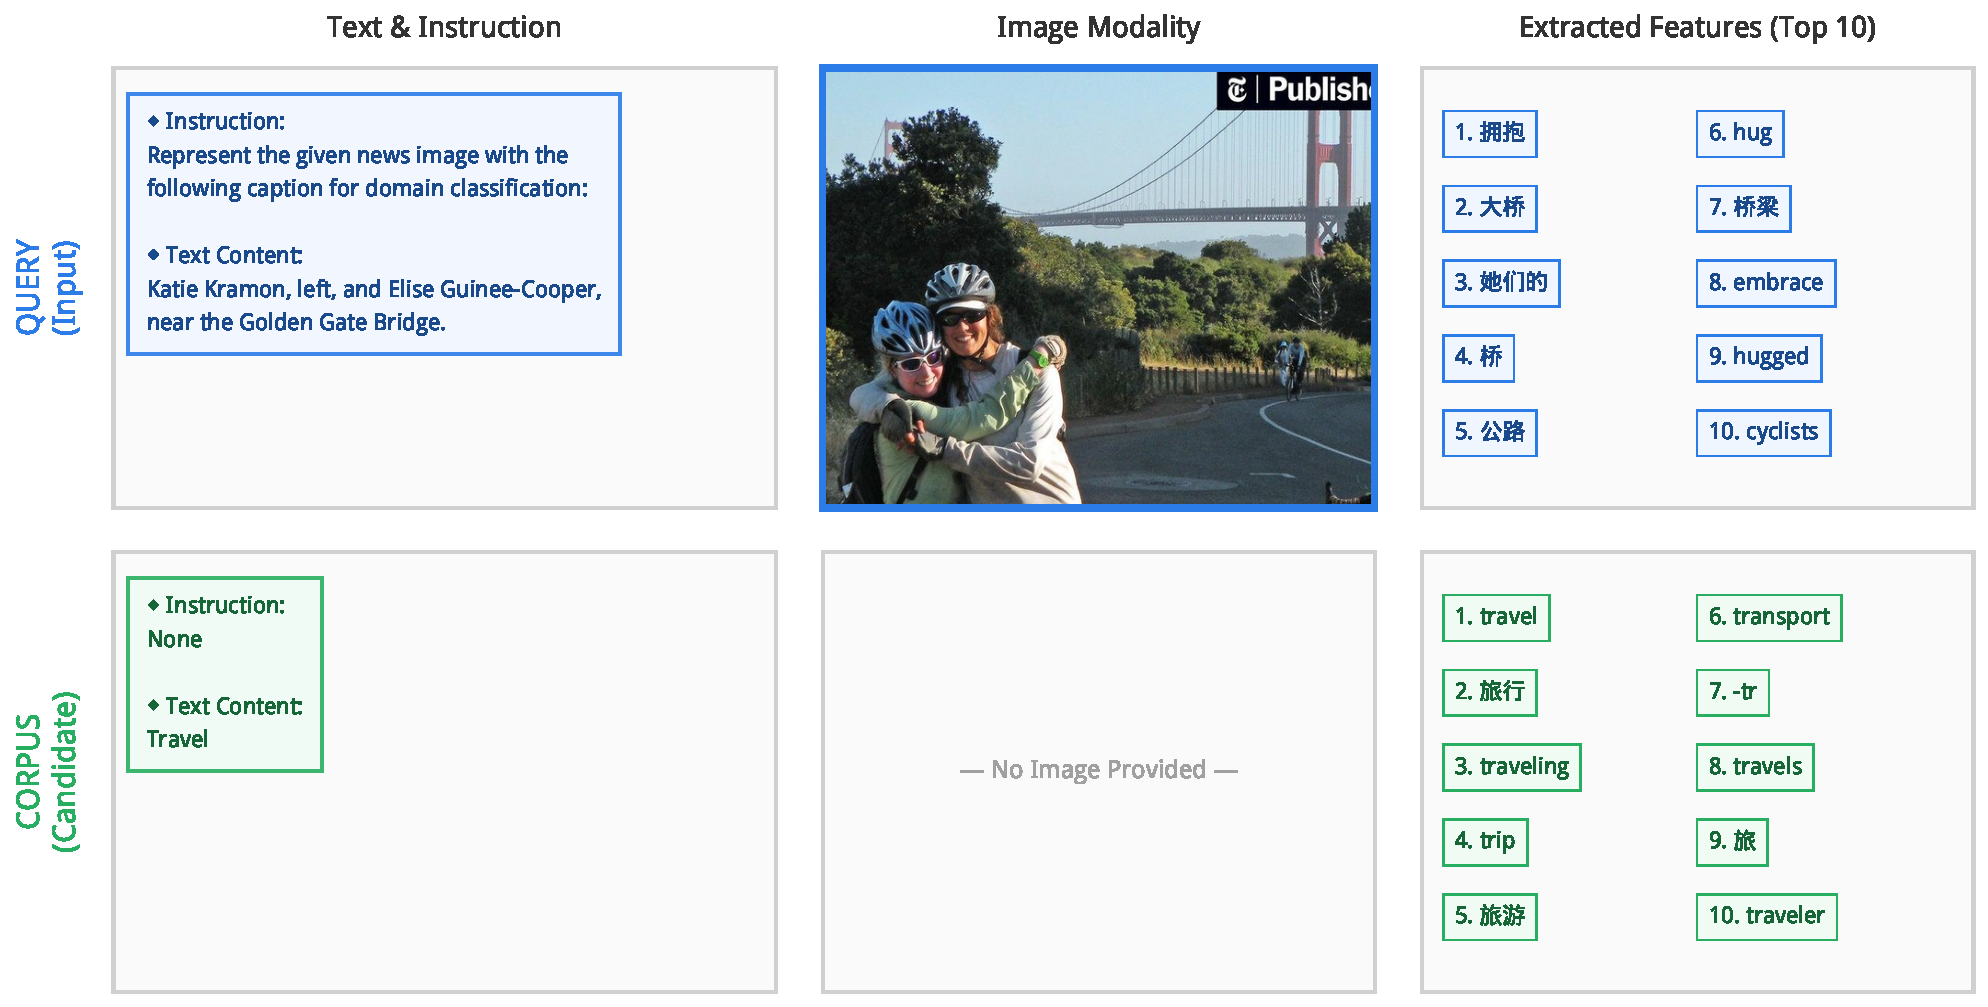
\includegraphics[width=\textwidth]{resources/case-study/CLS_N24News_case1.pdf}
\caption{Case study of \ours on classification (N24News). We visualize the top-10 activated sparse tokens.}
\label{fig:case-cls-n24news}
\end{figure*}


\begin{figure*}[htbp]
\centering
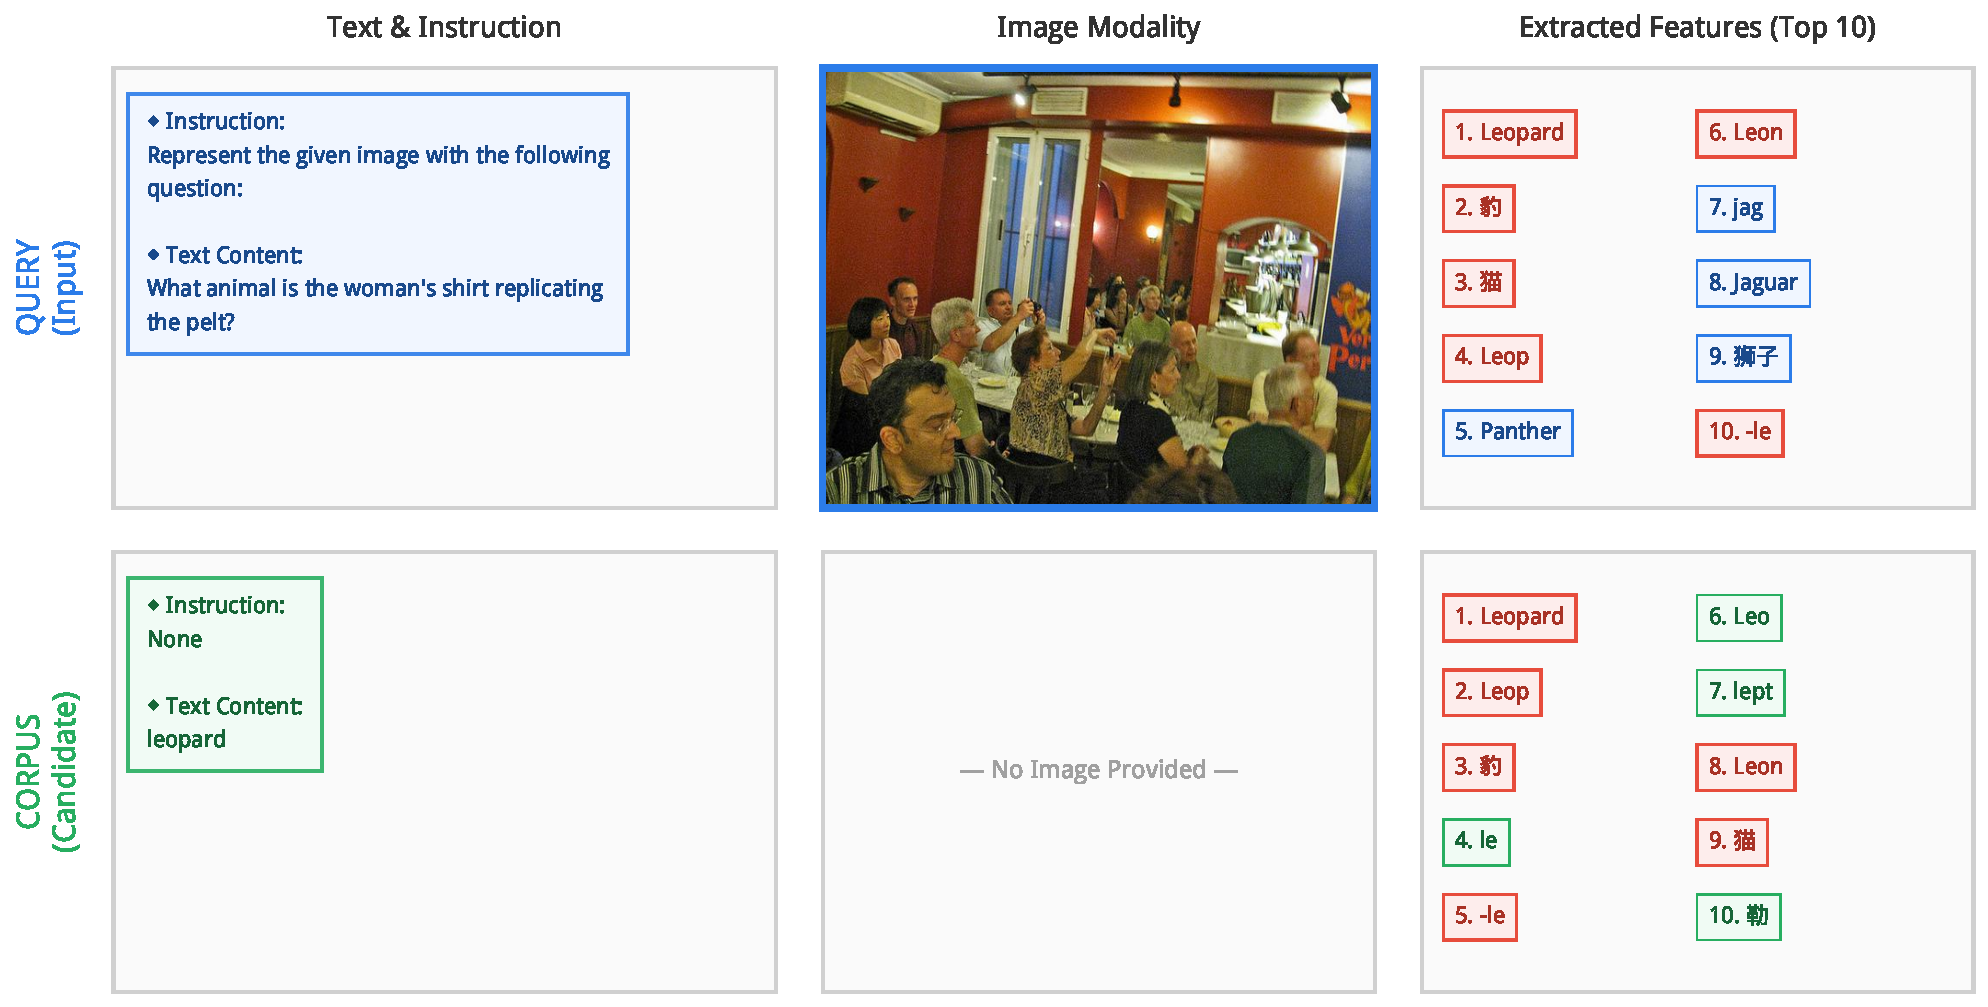
\includegraphics[width=\textwidth]{resources/case-study/QA_OK-VQA_case1.pdf}
\caption{Case study of \ours on question answering (OK-VQA). We visualize the top-10 activated sparse tokens.}
\label{fig:case-qa-okvqa}
\end{figure*}



\begin{figure*}[htbp]
\centering
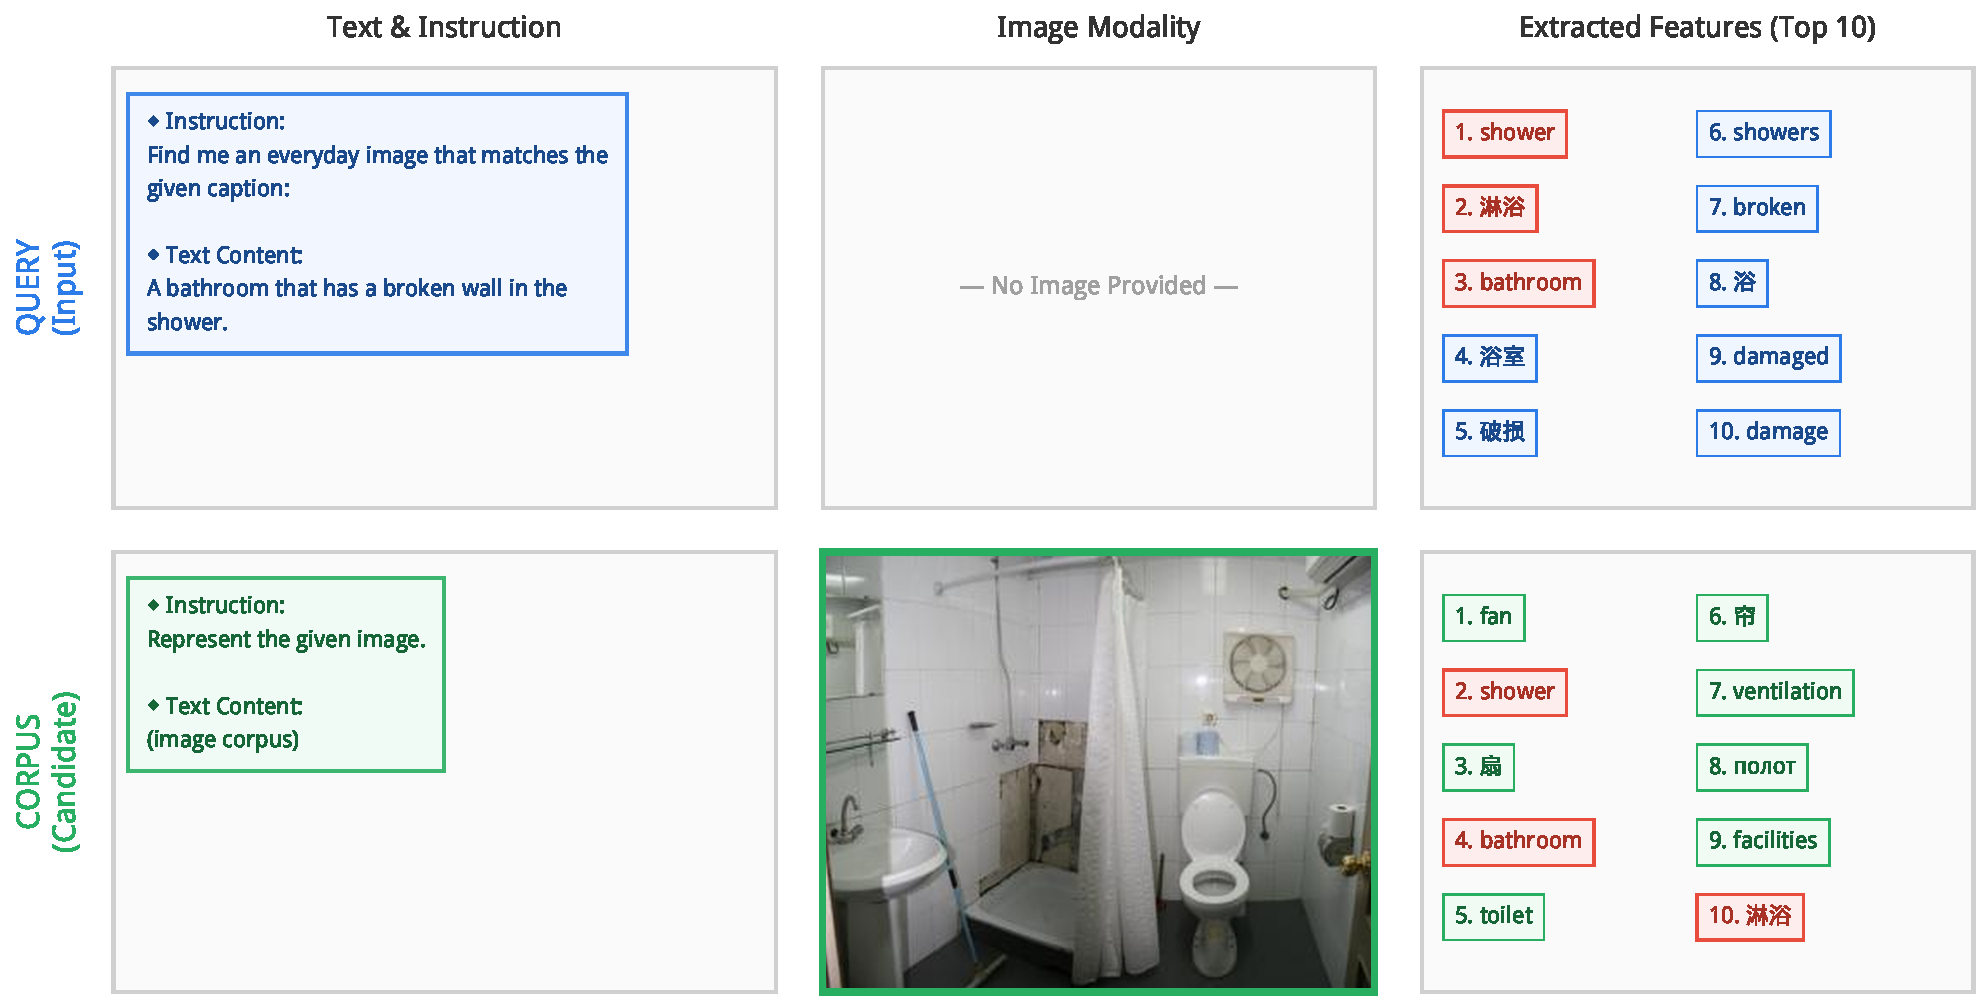
\includegraphics[width=\textwidth]{resources/case-study/RET_MSCOCO_t2i_case2.pdf}
\caption{Case study of \ours on text-to-image retrieval (MSCOCO). We visualize the top-10 activated sparse tokens.}
\label{fig:case-ret-mscoco-t2i}
\end{figure*}



\begin{figure*}[htbp]
\centering
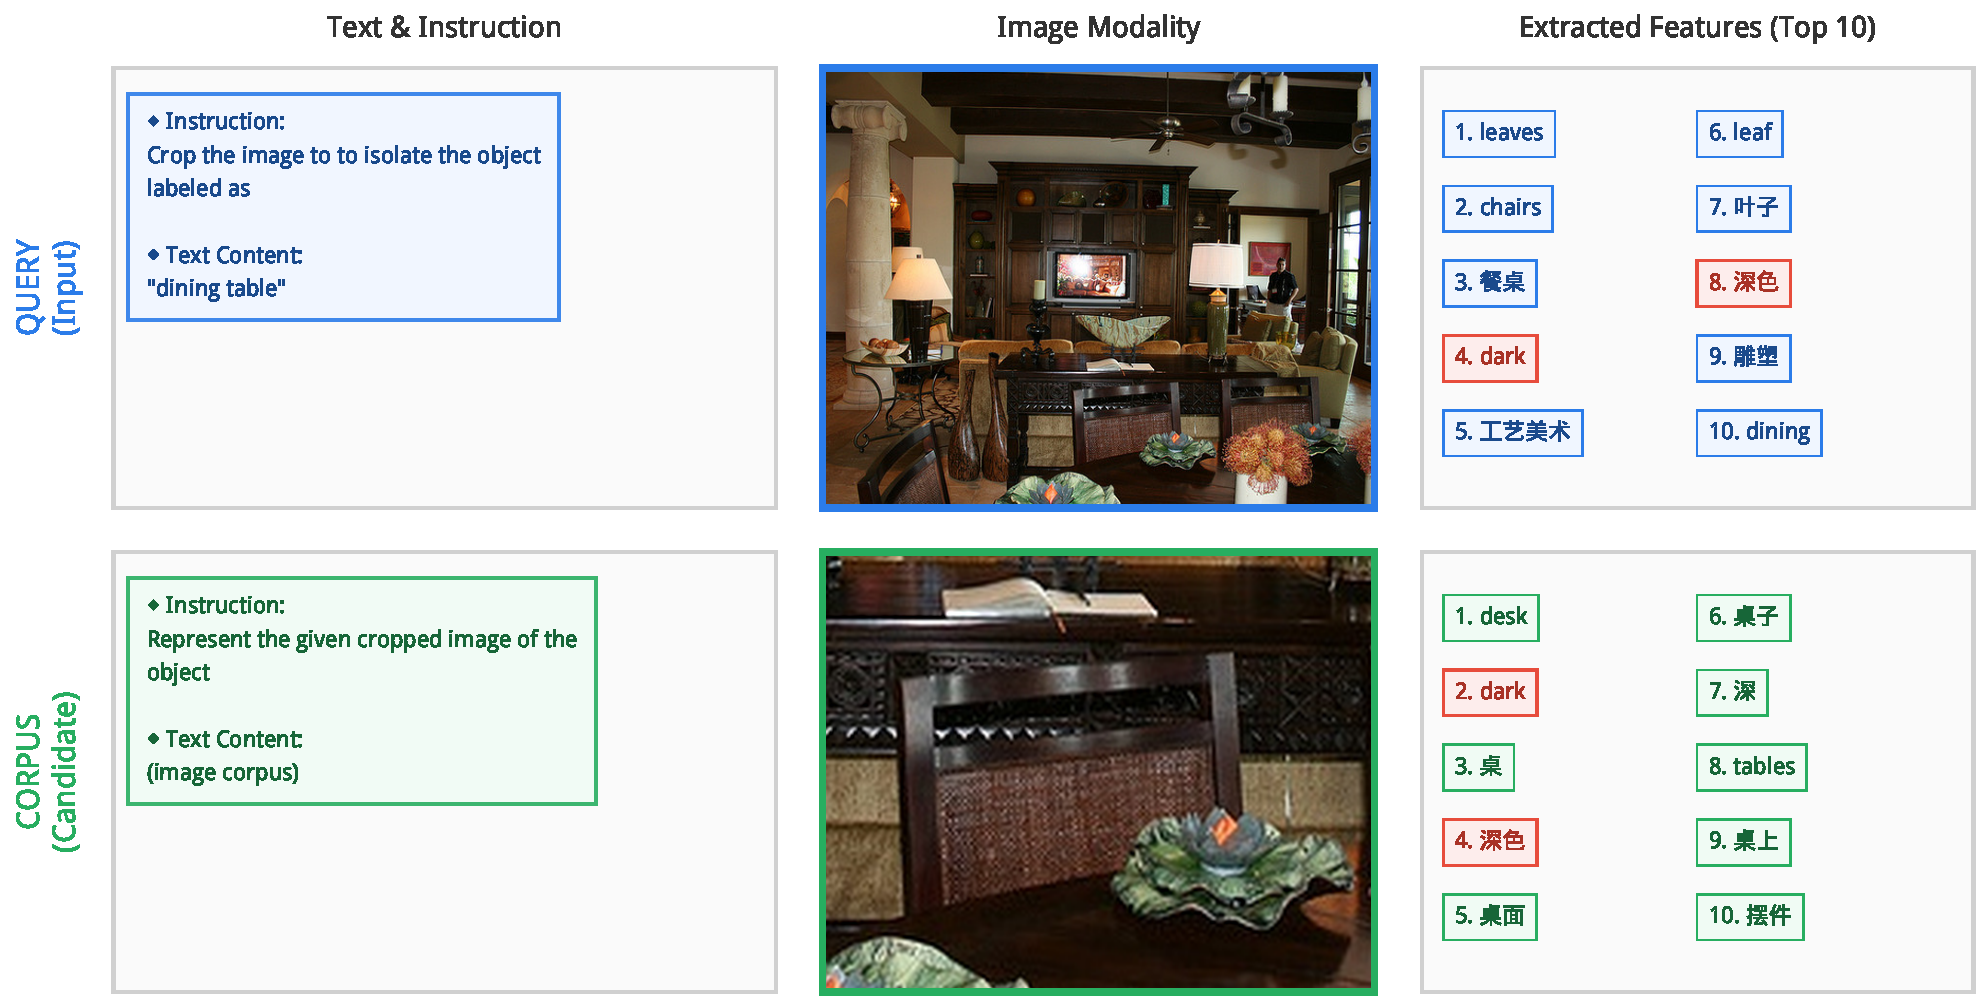
\includegraphics[width=\textwidth]{resources/case-study/GRD_MSCOCO_case1.pdf}
\caption{Case study of \ours on grounding (MSCOCO). We visualize the top-10 activated sparse tokens.}
\label{fig:case-grd-mscoco}
\end{figure*}
